% !TEX root = ../report.tex

\clearpage
\chapter{Pattern Documentation}
\label{ch:patterns}

\section{Client-Server}

% see https://docs.docker.com/engine/introduction/understanding-docker/

\begin{description}
\item [Traceability]~\\
The Client-Server pattern can be deducted from the online documentation\cite{dockerarchi}.

The Client-Server pattern can be deducted from the `What is Docker’s architecture?' section of the online documentation\cite{dockerarchi}.

\item [Source]~\\
Architectural patterns revisited -- a pattern language, P. 29 \cite{avgeriou2005architectural}

\item [Issue]~\\
For good interoperability, it should be possible for Docker containers to be started remotely. A single interface should be able to control containers on numerous hosts.

\item [Assumptions/Constraints]~

\item [Solution]~\\
Docker uses a Client-Server architecture. The client, a binary supplying a command-line interface, act as the primary interface for the user. The user enters commands into this client, which are then send to a server: the docker daemon. 


It should be possible for Docker containers to be controlled remotely and a single interface should be able to control containers on multiple hosts (e.g. in the cloud).

Additionally, certain operating systems lack the underlying technologies necessary for running containers. For those OSes, it should be possible to call remote daemons running on operating systems which are supported. % /WindowsBashing
% Me wantz to run on da windooowz, butz it aint got no cgroups

\item [Assumptions/Constraints]~
\begin{itemize}
\item The versions of the client binary and the server binary should match. Different versions can cause problems.
\item All the services offered by the daemon have to be made available to the client using a REST interface.
\end{itemize}

\item [Rationale] ~\\
The daemon is a background process, which supplies the requested services to the client. The daemon exposes a REST interface.

For Docker, the client can be configured to connect to other daemon processes than the one running on the local machine. It can be configured to connect to remote Docker daemons as well, allowing the user to issue commands to daemons running remotely.

%todo move above to architecture chapter 

By separating the client and server it is possible to use the same client to issue commands to different daemons, running on different hosts.
It is also possible to use the client on operating systems that do not support running containers.

\item [Implications]~\\
The use of the Client-Server pattern results in two different executable binaries: a daemon and a client. 


The use of a separated client handling the user interaction increases the modularity.
Furthermore, it increases the interoperability, since the client can send commands to daemons running on remote machines and the local machine.

All the services offered by the daemon have to be made available to the client using a REST interface.

It increases the interoperability, since the client can send commands to daemons running on remote machines and the local machine.

Additionally, the portability is increased, since the client can run on Operating System that cannot run containers themselves.


\item [Related Patterns]~\\


\end{description}

\section{Layers}
% see https://www.docker.com/sites/default/files/what-is-vm-diagram.png

% \begin{figure}[H]
% \centering
% 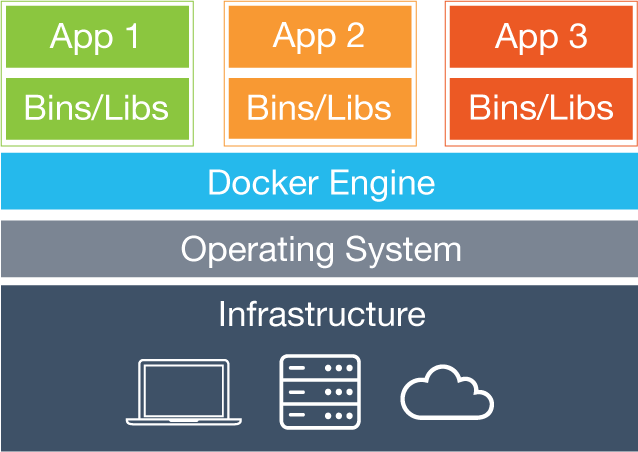
\includegraphics[scale=0.4]{5-patterns/images/what-is-vm-diagram.png}
% \caption{A layered overview of the Docker. Source \cite{whatisdocker}}
% \label{fig:layers-pattern}
% \end{figure}

\begin{description}
\item [Traceability]~\\
Layers is mentioned in the Docker architecture in the online documentation,
specifically in the explanation of Docker images\cite{dockerarchi}. Furthermore,
\cite{dockerimage} also elaborates on layers in the Docker images.

\item [Source]~\\
Architectural patterns revisited -- a pattern language, P. 29
\cite{avgeriou2005architectural}

\item [Issue]~\\
Docker emphasize on developing containerization with almost no overhead. Running
multiple instance of Docker containers with the same image may end up in high
overhead. A sharing and reuse mechanism must be implemented to prevent overhead
and to save more space or resource.

\item [Assumptions/Constraints]~\\
An application running in Docker container must has CLI\footnote{Command Line
Interface} (bash), as Docker image is a based on Linux distribution.

\item [Solution]~\\
Each Docker image consists of a stack of layers, which is read-only. The first
layer in the stack is a base image from Linux distribution. Docker also
implements copy-on-write strategy. In this strategy, system processes that need
the same data share the same instance of data rather than having their own. A
copy will be made when a specific system process makes a change to the data.

\item [Rationale] ~\\
Layers are very good in terms of sharing and reusability. In this way, overhead
can be avoided by sharing resources. A new image that uses same stack of layers
may reuse the layers rather than making a separate copy. This may result in
smaller size of Docker image.

\item [Implications]~\\
A Docker container will use Docker image as the base of it. This will remain as
read-only layers. Then, a Docker container will create another thin writable
layer on top of the image. Multiple containers that run based on the same Docker
image will not make their own copy of the image to prevent duplication. This
will end up in more efficient memory allocation.

\item [Related Patterns]~\\
\begin{itemize}
	\item Client-server
	\item Shared repository
\end{itemize}
\end{description}

% \clearpage


\section{Shared repository}
%\textit{Can we consider the docker registry a shared repository?}
% Schemas
%http://fr.slideshare.net/Docker/https-dldropboxusercontentcomu20637798docker-meetup-freiburg
% http://blog.octo.com/en/docker-registry-first-steps/   http://fr.slideshare.net/egorpushkin/docker-demo   
% Because of Pull/¨Push can we talk about Pattern publish suscribe ?   Asynhcronous Queuing ?

The docker registry is considered as a Shared Repository. \\
Two alternatives exist:DockerHub and Docker Trusted Registry. \\

Docker has a feature wich can be configured : the Notification Sytem which makes the Shared Repository an active Repository.
\textit{https://docs.docker.com/registry/notifications/}

\begin{description}
\item[Traceability]~\\
The Shared Repository pattern can be deducted from the online documentation : \textit{https://docs.docker.com/registry/}
\quote{"The Registry is a stateless, highly scalable server side application that \textbf{stores} and lets you \textbf{distribute} Docker images. A registry is a storage and content delivery system."} 
% File store.go , registry.go

\item[Source]~\\
%\EAA, P.322 \cite{eaa}\\
Architectural Pattern Revisited - A Pattern Language, P.13 \cite{avgeriou2005architectural}

\item[Issue]~\\
Docker provided a way for the user to conrol the storage and distribution of images.
User need to be alerted of new events happening in the registry through notifications. % Develop ?

\item[Assumptions/ Contrainst]~\\

\item[Solution]~\\ %how does it work ?
\quote{Users interact with a registry by using docker push and pull commands.}

\item[Rationale]~\\ % in which way this pattern helps Docker? What is the goal ? KD
By using the Shared Repository Pattern 

\end{description}

\subsection{Event-Driven Messaging}

\begin{description}

\item[Traceability]~\\
The notification mechanism of the Docker Registry uses the Even-Driven Messaging Pattern.

\item[Source]~\\
%\textit{http://soapatterns.org/design_patterns/event_driven_messaging}

\item[Issue]~\\ The user wants to be alerted about certain events occuring in his registry.
The notification system needs a mechanism in order to send the events to the user.

\item[Assumptions/Contrainst]~\\ This pattern is used at a lower level in the Docker Registry/Active Repository Pattern.

\item[Solution]~\\

\item[Rationale]~\\ 
\quote { Notifications are sent to endpoints via HTTP requests. Each configured endpoint has isolated queues, retry configuration and http targets within each instance of a registry. When an action happens within the registry, it is converted into an event which is dropped into an inmemory queue. When the event reaches the end of the queue, an http request is made to the endpoint until the request succeeds. The events are sent serially to each endpoint but order is not guaranteed. }

\end{description}

\begin{figure}[H]
\centering
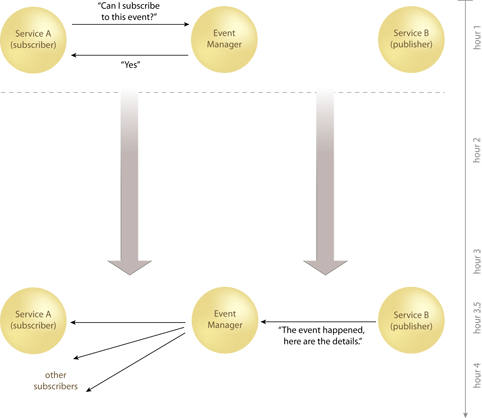
\includegraphics{images/EDM.png}
\caption{Event-Driven Messaging}
\label{fig:event-driven}
\end{figure}

\subsection{Direct Authentication/ Brokered Authentication}

\begin{description}

\item[Traceability]~\\
The Direct Authentication pattern can be deducted from the source code through the "auth.go" file from the Docker Github Repository. \\
The notification mechanism of the Docker Registry uses this pattern.

\item[Source]~\\
\textit{https://msdn.microsoft.com/en-us/library/ff647715.aspx} \\
%http://soapatterns.org/design_patterns/direct_authentication
%https://docs.docker.com/registry/spec/auth/token/


\item[Issue]~\\ The Docker Registry needs an authentication system in order to ensure security for the user through a login.
%The access to the Docker Registry is managed by an authentication system ...

\item[Assumptions/Contrainst]~\\ 

\item[Solution]~\\

\item[Rationale]~\\ 


\end{description}

\section{Plugin}
\label{sec:pattern-plugin}
%TODO image
\begin{description}

\item [Traceability]~\\
The existence of Docker Plugins becomes apparent from it's documentation at \cite{dockerplugindocs}.

Additionally, the directories \verb|docker/pkg/plugins/| \footnote{\url{https://github.com/docker/docker/tree/master/pkg/plugins}} and \verb|  docker/daemon/graphdriver/plugin.go| \footnote{\url{https://github.com/docker/docker/blob/master/daemon/graphdriver/plugin.go}} (among others) in the project's repository contain the code for discovering plugins and the interfaces the plugins should implement.

\item [Source]~\\
Patterns of Enterprise Application Architecture, P. 499 \cite{eaa}

\item [Issue]~\\
The users of Docker want to have customization, by extending Docker with third party custom-built tools. This customization means that third parties should be able to write plugins that extend Docker's core functionality.\cite{dockerpluginblog}

The implementation of such plugins is only available at runtime.

\item [Assumptions/Constraints]~
\begin{itemize}
\item Plugins can only extends the functionality of the components of Docker, that have an interface that plugins can implement.
\end{itemize}


\item [Solution]~\\
Docker uses the Plugin pattern to link the implementation of the interfaces of several extendable components with third-party implementation at runtime.

\item [Rationale] ~\\ % https://docs.docker.com/engine/extend/plugin_api/
Docker discovers plugins by looking for .sock, .spec or .json files in the plugin directories on the host system. These files describe how Docker can communicate with the plugins using the REST API (usually via a Unix socket).

The plugins themselves run as separate processes on the same host as the Docker daemon and implement an HTTP server listening for requests from the Docker daemon. After a user requires a plugin (this is indicated e.g. as a command-line parameter when starting a container using the Docker client) Docker uses the discovery algorithm (see also Section~\ref{sec:processplugins}). After that, Docker sends a handshake to the plugin and the plugin returns a list of which subsystems this plugin implements.


For these subsytems Docker will replace the default implementation by a Proxy, that forwards all calls over the REST interface to the plugin process.

\item [Implications]~\\
The use of the Plugins pattern means that the adaptability increases. 

\item [Related Patterns]~
\begin{itemize}
\item Proxy
\end{itemize}
\end{description}

\section{Proxy}
\begin{description}

\item [Traceability]~\\
The use of the \pattern{proxy} pattern becomes apparent from the source code in the repository on GitHub.
For example, the proxy for the Volumes plugin can be found in \verb|docker/daemon/graphdriver/proxy.go| \footnote{\url{https://github.com/docker/docker/blob/master/daemon/graphdriver/proxy.go}}.

\item [Source]~\\
Pattern-oriented Software Architecture - Volume 4, P.290 \cite{wiley4}

\item [Issue]~\\
The plugins are separate processes than the daemon and are only available at runtime. Therefore, it is impossible for the daemon process to access the services of the plugins directly.
% issue also for comms between client-server ??

\item [Assumptions/Constraints]~
\begin{itemize}
\item The plugins have to implement a server listening for requests from the daemon.
\end{itemize}

\item [Solution]~\\
Let the daemon only communicate with the plugins through a proxy. This proxy implements all the `housekeeping' functionality, like sending API requests and authentication. It has the same interface as the plugin. \\
Whenever a call is done from the daemon to the plugin, it goes via the proxy, which communicates this call using a REST API to the plugin process.

\item [Rationale] ~\\ 
Using the \pattern{proxy} pattern allows the daemon to communicate with the plugins, without requiring direct access to these plugins. \\
Also, because the subsystem component has the same interface as its proxy, the implementation of software using this component does not depend on whether the proxy is used or the original subsystem. 

\item [Implications]~\\
The use of the \pattern{proxy} pattern allows communication with the plugins, which increases the extendability. 
Because the communication with the process is not direct, there is some performance overhead.
%TODO: what about portability??

\item [Related Patterns]~
\begin{itemize}
\item Plugin
\end{itemize}

\end{description}

